\chapter{មូលដ្ឋានគ្រឹះខ្លះៗនៃគណិតវិទ្យា}
\section{ស្វ័យគុណ}
\quad ស្វ័យគុណត្រូវបានប្រើជាញឹកញាប់នៅក្នុងរូបវិទ្យា ពេលយើងសរសេរ $3^{4}$ ដែល $4$ ហៅថាស្វ័យគុណ ហើយ $3$ ជាគោល។
\begin{formula}
	\begin{enumerate}[m,2]
		\item $a^{0}=1\quad \left(a\ne 0\right)$
		\item $a^{n}=a\times a\times a \times \cdots \times a\quad\left(a\ne 0\right)$
%		\emph{ឧទាហរណ៍ទី១ៈ} $10^{4}=10\times10\times10\times10=10000$\\
%		\emph{ឧទាហរណ៍ទី២ៈ} $10^{2}=10\times10=100$
		\item $a^{-n}=\frac{1}{a^{n}}\quad \left(a\ne 0\right)$
		\item $a^{m}\cdot a^{n}=a^{m+n}\quad \left(a\ne 0, n\ne 0, m\ne 0\right)$
		\item $\frac{a^{m}}{a^{n}}=a^{m-n}\quad \left(a\ne 0, n\ne 0, m\ne 0\right)$
		\item $\left(a\cdot b\right)^{n}=a^{n}\cdot b^{n}\quad \left(n\ne 0\right)$
		\item $\left(a^{m}\right)^{n}=\left(a^{n}\right)^{m}=a^{m\cdot n}\quad \left(a\ne 0, n\ne 0, m\ne 0\right)$
		\item $\left(\frac{a}{b}\right)^{n}=\frac{a^{n}}{b^{n}}\quad \left(b\ne 0, n\ne 0\right)$
		\item $\sqrt[n]{a^{m}}=a^{\frac{m}{n}}$ និង $\sqrt[n]{a}\times\sqrt[n]{b}=\sqrt[n]{a\times b}$
		\item $\frac{\sqrt[n]{a}}{\sqrt[n]{b}}=\sqrt[n]{\frac{a}{b}}$
	\end{enumerate}
\end{formula}
\section{ឯកលក្ខណៈភាពសំខាន់ៗ}
\begin{formula}
	\begin{enumerate}[m,2]
		\item $\left(a+b\right)^{2}=a^{2}+2ab+b^{2}$
		\item $\left(a-b\right)^{2}=a^{2}-2ab+b^{2}$
		\item $\left(a+b\right)^{3}=a^{3}+3a^{2}b+3ab^{2}+b^{3}$
		\item $\left(a+b\right)^{3}=a^{3}-3a^{2}b+3ab^{2}-b^{3}$
		\item $a^{2}-b^{2}=\left(a-b\right)\left(a-b\right)$
		\item $a^{2}+b^{2}=\left(a+b\right)^{2}-2ab$
		\item $a^{3}-b^{3}=\left(a-b\right)\left(a^{2}+ab+b^{2}\right)$
		\item $a^{3}+b^{3}=\left(a+b\right)\left(a^{2}-ab+b^{2}\right)$
	\end{enumerate}
\end{formula}
\section{លក្ខណៈនៃប្រភាគពីរស្មើគ្នា}
\begin{generality}
	ឧបមាថាយើងមានប្រភាគពីរស្មើគ្នា $\frac{a}{b}=\frac{c}{d}$។ យើងអាចសរសេរបានដូចខាងក្រោមៈ
	\begin{enumerate}[m,2]
		\item $\frac{d}{b}=\frac{c}{a}$ (ប្តូរតួចុង)
		\item $\frac{a}{c}=\frac{b}{d}$ (ប្តូរតួមធ្យម)
		\item $a\cdot d=b\cdot c$ (ផលគុណតួចុងស្មើនឹងផលគុណតួមធ្យម)
		\item $\frac{a}{b}=\frac{c}{d}=\frac{a\pm c}{b\pm d}$ (លក្ខណៈផលធៀបស្មើតគ្នា)
	\end{enumerate}
\end{generality}
\section{សមីការបន្ទាត់}
\begin{formula}
	សមីការបន្ទាត់មានរាង $y=ax+b$ ដែល $a$ ជាមេគុណប្រាប់ទិស និង $b$ ជាចំនួនថេរ។ បើ $b=0$ នោះសមីការបន្ទាត់មានរាង $y=ax$ គេថាបន្ទាត់កាត់តាមគល់ $0$។
	\begin{align*}
		\text{មេគុណប្រាប់ទិសនៃបន្ទាត់គឺ}\quad :&\quad a=\frac{\Delta y}{\Delta x}=\frac{y_{2}-y_{1}}{x_{2}-x_{1}}
	\end{align*}
\end{formula}
\section{ទម្រង់ស្តង់ដានៃស្វ័យគុណ}
 ទម្រង់ស្តង់ដានៃស្វ័យគុណរបស់ចំនួនមួយគឺជាផលគុណនៃចំនួន $A$ ដែល $1\le A<10$ នឹងស្វ័យគុណ $10$។ ដូចនេះទម្រង់ស្តង់ដាមានរាង $A\times10^{n}$ ដែល $1\le A<10$ ហើយ $n$ ជាចំនួនគត់រុឺឡាទីប។
 \begin{example}
 	សរសេរចំនួនខាងក្រោមជាទម្រង់ស្តង់ដាៈ
 	\begin{enumerate}[k,2]
 		\item $550~000~000=55\times10^{7}$
 		\item $0.000~000~343=343\times10^{-9}$
 		\item $0.000~000~000~004mm=4\times10^{-12}mm$
 		\item $300~000km/s=3\times10^{5}km/s$
 	\end{enumerate}
 \end{example}
\section{ទ្រឹស្តីបទកូសុីនុស និងសុីនុស}
\begin{theorem}
	\begin{multicols}{2}
		\emph{\kml $\bullet$ ទ្រឹស្តីបទកូសុីនុស}
		\begin{align*}
		a^{2}=b^{2}+b^{2}-2bc\cos\alpha\\
		b^{2}=a^{2}+c^{2}-2ac\cos\beta\\
		c^{2}=a^{2}+b^{2}-2ab\cos\gamma\\
		\end{align*}
		\emph{\kml $\bullet$ ទ្រឹស្តីបទសុីនុស}
		\begin{align*}
		\frac{a}{\sin \alpha}=\frac{b}{\sin \beta}=\frac{c}{\sin \gamma}=2R\\ \text{$R$ ជាកាំរង្វង់ចរឹកក្រៅត្រីកោណ}
		\end{align*}
		\emph{\kml $\bullet$ ផលបូកមុំក្នុងនៃត្រីកោណៈ} $\alpha + \beta + \gamma=180^\circ$
		\begin{figure}[H]
			\centering
			\begin{tikzpicture}[scale=1]
			\RectTri{(0,4)}{(1,0)}{5cm}
			\end{tikzpicture}
			\caption{ត្រីកោណនៃទ្រឹស្តីបទកូសុីនុស និងសុីនុស}
		\end{figure}
	\end{multicols}
\end{theorem}
\section{ផលគុណស្កាលែនៃពីរវុិចទ័រ}
	\begin{multicols}{2}
	\emph{\kml ផលគុណស្កាលែនៃពីរវុិចទ័រៈ} បើគេមានវុិចទ័រពីរ $\overrightarrow{A}$ និង $\overrightarrow{B}$ ដែលផ្គុំគ្នាបានមុំ $\theta$ ដូចរូបខាងស្តាំ។ \newline
	នោះគេអាចសរសេរ
		\begin{align*}
			\text{គេសរសេរ}\quad :&\quad\overrightarrow{A}\cdot\overrightarrow{B}=\abs{\overrightarrow{A}}\abs{\overrightarrow{B}}\cos\theta\\
			\text{ម្យ៉ាងទៀត}\quad :&\quad \quad\overrightarrow{A}\cdot\overrightarrow{B}=AB\cos\theta\\
			\text{បើ}\quad :&\quad\overrightarrow{A}\cdot\overrightarrow{B}=0 \quad \text{នោះ}\quad \overrightarrow{A}\perp\overrightarrow{B}\\
			\text{ដែល}\quad :&\quad  \abs{\overrightarrow{A}}=A\quad \text{និង}\quad \abs{\overrightarrow{B}}=B\quad \text{ហៅថាណម ឬប្រវែងនៃវុិចទ័រ}
		\end{align*}
		\begin{figure}[H]
			\centering
			\begin{tikzpicture}[scale=1.3]
			\begin{scope}
			\coordinate (O) at (0,0);
			\coordinate (A) at (2,2);
			\coordinate (B) at (3,0);
			\coordinate (C) at (4,2);
			\draw [->] (O) -- (A);
			\draw [->] (O) -- (B);
			\draw [dashed] (A) -- (2,0);
			\coordinate[label=above:$\overrightarrow{A}$] (A) at (A);
			\coordinate[label=below:$\overrightarrow{B}$] (B) at (B);
			\pic [draw, -, "$\theta$", angle eccentricity=1.5] {angle = B--O--A};
			\end{scope}
			\end{tikzpicture}
			\caption{ផលគុណស្កាលែនៃពីរវុិចទ័រ}
		\end{figure}
	\end{multicols}
\section{ធរណីមាត្រក្នុងប្លង់ និងអនុគមន៍ត្រីកោណមាត្រ}
\subsection{ការេ}
គេមានការេ $ABCD$ ដែលមានជ្រុង $a$ ដូចរូប។ គេបាន
\begin{multicols}{2}
	\begin{align*}
		\text{ជ្រុង}\quad :&\quad \abs{AB}=\abs{BC}=\abs{CD}=\abs{DA}=a\\
		\text{អង្កត់ទ្រូង}\quad :&\quad \abs{AC}=\abs{BD}=a\sqrt{2}\\
		\text{ពីកំពូលទៅផ្ចិត}\quad :&\quad \abs{AO}=\abs{BO}=\abs{CO}=\abs{DO}=\frac{a\sqrt{2}}{2}\\
		\text{បរិមាត្រ}\quad :&\quad P=4a\\
		\text{ផ្ទៃក្រឡា}\quad :&\quad S=a\cdot a=a^{2}
	\end{align*}
	\begin{figure}[H]
		\centering
		\begin{tikzpicture}
			\begin{scope}
				\coordinate[label=below left:$A$] (A) at (0,0);
				\coordinate[label=below right:$B$] (B) at (3,0);
				\coordinate[label=above right:$C$] (C) at (3,3);
				\coordinate[label=above left:$D$] (D) at (0,3);
				\coordinate[label=below:$O$] (O) at (1.5,1.5);
				\coordinate[label=above:$a$] (a) at (1.5,3);
				\draw (A)--(B)--(C)--(D)--cycle;
				\draw[dashed] (A)--(C);
				\draw[dashed] (B)--(D);
			\end{scope}
		\end{tikzpicture}
		\caption{ការេ}
	\end{figure}
\end{multicols}
\subsection{ចតុកោណកែង}
គេមានចតុកោណកែង $ABCD$ ដែលមានទទឹង​ $a$ និងបណ្តោយ $b$ ដូចរូប។ គេបាន
\begin{multicols}{2}
	\begin{align*}
	\text{ជ្រុង}\quad :&\quad \abs{AD}=\abs{BC}=a,~\abs{AB}=\abs{DC}=b\\
	\text{អង្កត់ទ្រូង}\quad :&\quad \abs{AC}=\abs{BD}=\sqrt{a^{2}+b^{2}}\\
	\text{បរិមាត្រ}\quad :&\quad P=2a+2b\\
	\text{ផ្ទៃក្រឡា}\quad :&\quad S=a\cdot b
	\end{align*}
	\begin{figure}[H]
		\centering
		\begin{tikzpicture}
		\begin{scope}
		\coordinate[label=below left:$A$] (A) at (0,0);
		\coordinate[label=below right:$B$] (B) at (4,0);
		\coordinate[label=above right:$C$] (C) at (4,3);
		\coordinate[label=above left:$D$] (D) at (0,3);
		\coordinate[label=below:$O$] (O) at (2,1.5);
		\coordinate[label=above:$b$] (b) at (2,3);
		\coordinate[label=right:$a$] (a) at (4,1.5);
		\draw (A)--(B)--(C)--(D)--cycle;
		\draw[dashed] (A)--(C);
		\draw[dashed] (B)--(D);
		\end{scope}
		\end{tikzpicture}
		\caption{ចតុកោណកែង}
	\end{figure}
\end{multicols}
\subsection{ប្រភេទនៃត្រីកោណ}
\begin{enumerate}[m]
	\item \emph{\kml ត្រីកោណសាមញ្ញ}
	\begin{multicols}{2}
		គេមានត្រីកោណ $ABC$ ដែលមានកម្ពស់ $h$ ដូចរូប។
		\begin{align*}
		\text{យើងបាន}\quad :&\quad \text{ផ្ទៃក្រឡា}=\frac{\text{បាត}\times \text{កម្ពស់}}{2}\\
		\text{គេអាចសរសេរ}\quad :&\quad S=\frac{AC\times h}{2}\\
		\text{មុំ}\quad :&\quad \alpha + \beta + \theta =180^\circ
		\end{align*}
			\begin{figure}[H]
			\centering
			\begin{tikzpicture}
			\begin{scope}
				\coordinate[label=below left:$A$] (A) at (-1,0);
				\coordinate[label=above right:$B$] (B) at (4,3);
				\coordinate[label=below right:$C$] (C) at (6,0);
				\coordinate[label=below:$H$] (H) at (4,0);
				\coordinate[label=right:$h$] (h) at (4,1.5);
				\draw (A)--(B)--(C)--cycle;
				\draw (B)--(H);
			\end{scope}
			\end{tikzpicture}
			\caption{ត្រីកោណសាមញ្ញ}
		\end{figure}
	\end{multicols}
	\item \emph{\kml ត្រីកោណកែង} គេមានត្រីកោណកែង $ABC$ ដែលមានកម្ពស់ $h$ ដូចរូប។
	\begin{multicols}{2}
		\begin{align*}
			\text{យើងបានក្រឡាផ្ទៃ}\quad :&\quad  S=\frac{AC\times h}{2}\\
			\text{មុំ}\quad :&\quad \alpha + \beta + \theta =180^\circ\\
			\text{ដែល}\quad :&\quad \theta = 90^\circ
		\end{align*}
		\begin{figure}[H]
			\centering
			\begin{tikzpicture}
				\begin{scope}
					\coordinate[label=below left:$A$] (A) at (-1,0);
					\coordinate[label=above right:$B$] (B) at (4,3);
					\coordinate[label=below right:$C$] (C) at (4,0);
%					\coordinate[label=below:$H$] (H) at (4,0);
					\coordinate[label=right:$h$] (h) at (4,1.5);
					\draw (A)--(B)--(C)--cycle;
%					\draw (B)--(H);
				\end{scope}
			\end{tikzpicture}
			\caption{ត្រីកោណកែង}
		\end{figure}
	\end{multicols}
	\item \emph{\kml ត្រីកោណសមបាត} គេមានត្រីកោណសមបាត $ABC$ ដូចរូប។ យើងបាន
	\begin{multicols}{2}
		\begin{align*}
			\text{ជ្រុង}\quad :&\quad \abs{AB}=\abs{BC}=\abs{AC}\times\frac{\sqrt{2}}{2}\\
			\text{កម្ពស់}\quad :&\quad \abs{BH}=\abs{AH}=\abs{HC}=\frac{AC}{2}\\
			\text{មុំ}\quad :&\quad \alpha + \beta + \theta =180^\circ\\
			\text{ដែល}\quad :&\quad \theta = \beta = 45^\circ
		\end{align*}
		\begin{figure}[H]
			\centering
			\begin{tikzpicture}
				\begin{scope}
				\coordinate[label=below left:$A$] (A) at (0,0);
				\coordinate[label=above right:$B$] (B) at (3,3);
				\coordinate[label=below right:$C$] (C) at (6,0);
				\coordinate[label=below:$H$] (H) at (3,0);
				\coordinate[label=right:$h$] (h) at (3,1.5);
				\draw (A)--(B)--(C)--cycle;
				\draw (B) -- (H);
				\end{scope}
			\end{tikzpicture}
			\caption{ត្រីកោណសមបាត}
		\end{figure}
	\end{multicols}
	\item \emph{\kml ត្រីកោណសម័ង្ស} គេមានត្រីកោណសម័ង្ស $ABC$ ដូចរូប។ យើងបានៈ
		\begin{multicols}{2}
			\begin{align*}
			\text{ជ្រុង}\quad :&\quad \abs{AB}=\abs{BC}=\abs{AC}=a\\
			\text{កម្ពស់}\quad :&\quad \abs{BH}=\frac{a\sqrt{3}}{2}\\
			\text{មុំ}\quad :&\quad \alpha + \beta + \theta =180^\circ\\
			\text{ដែល}\quad :&\quad \theta = \beta = \alpha=60^\circ
			\end{align*}
			\begin{figure}[H]
				\centering
				\begin{tikzpicture}
				\begin{scope}
				\coordinate[label=below left:$A$] (A) at (0,0);
				\coordinate[label=above right:$B$] (B) at (2,4);
				\coordinate[label=below right:$C$] (C) at (4,0);
				\coordinate[label=below:$H$] (H) at (2,0);
				\coordinate[label=right:$h$] (h) at (2,1.5);
				\coordinate[label=right:$a$] (a) at (3.3,1.5);
				\draw (A)--(B)--(C)--cycle;
				\draw (B) -- (H);
				\end{scope}
				\end{tikzpicture}
				\caption{ត្រីកោណសមបាត}
			\end{figure}
		\end{multicols}
\end{enumerate}
\subsection{រង្វង់}
រង្វង់មួយមានផ្ចិត $O$ កាំ $R$ និងអង្កត់ផ្ចិត $D$ ដូចរូប
\begin{multicols}{2}
	\begin{align*}
	\text{អង្កត់ផ្ចិត}\quad :&\quad D=R+R=2R\\
	\text{បរិមាត្រ}\quad :&\quad P=\pi D=2\pi R\\
	\text{ក្រឡាផ្ទៃ}\quad :&\quad S=\pi R^{2}=\pi\frac{D^{2}}{4}
	\end{align*}
	\begin{figure}[H]
		\centering
		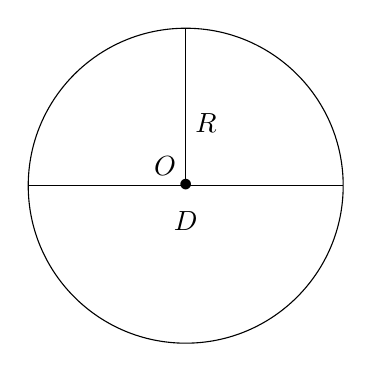
\begin{tikzpicture}
			\begin{scope}
				\coordinate[label=above left:$O$] (O) at (2,2);
				\coordinate[label=below:$D$] (D) at (2,1.8);
				\coordinate[label=right:$R$] (R) at (2,2.8);
				\draw (O) circle (2cm);
				\draw (O) -- (2,4);
				\draw (0,2) -- (4,2);
				\node at (O) {$\bullet$};
			\end{scope}
		\end{tikzpicture}
		\caption{រង្វង់}
	\end{figure}
\end{multicols}
\subsection{គូប}
គូបមួយមានទ្រនុង $a$ ដូចរូប។ យើងបានមាឌរបស់វាគឺ $V=a\cdot a\cdot a=a^{3}$
\begin{figure}[H]
	\centering
	\begin{tikzpicture}
	\pic at (-3,-2) {annotated cubic={width=20, height=20, depth=20, units=cm}};
	\end{tikzpicture}
	\caption{គូប}
\end{figure}
\subsection{ប្រលេពីប៉ែតកែង}
ប្រលេពីប៉ែតកែងមួយមានទ្រនុង $a$ បណ្តោយ $b$ និងកម្ពស់ $h$ ដូចរូប។ យើងបានមាឌរបស់វាគឺ $V=a\cdot b\cdot h$
\begin{figure}[H]
	\centering
	\begin{tikzpicture}
	\pic at (0,0) {annotated prole={width=30, height=10, depth=20, units=cm}};
	\end{tikzpicture}
	\caption{ប្រលេពីប៉ែតកែង}
\end{figure}
\subsection{សុីឡាំង}
សុីឡាំងមួយមានមុខកាត់ជារង្វង់ដែលមានកាំ $R$ និងកម្ពស់ $h$ ដូចរូប។ យើងបានមាឌ $V=S\cdot h=\pi R^{2}h$
\begin{figure}[H]
	\centering
	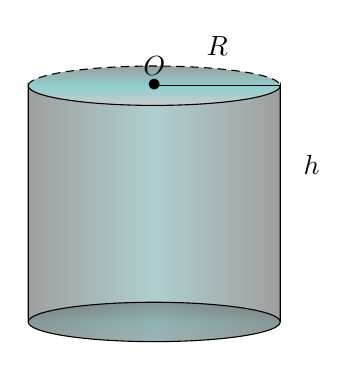
\begin{tikzpicture}[yscale=.5, xscale=.8]
		\coordinate[label=above:$O$] (O) at (0,0);
		\fill [top color=gray!50!black,bottom color=gray!10,middle color=cyan,shading=axis,opacity=0.25] (0,0) circle (2cm and 0.5cm);
		\fill [left color=gray!50!black,right color=gray!50!black,middle color=cyan!50,shading=axis,opacity=0.25] (2,0) -- (2,-6) arc (360:180:2cm and 0.5cm) -- (-2,0) arc (180:360:2cm and 0.5cm);
		\fill [top color=gray!90!,bottom color=gray!2,middle color=cyan!30,shading=axis,opacity=0.25] (0,-6) circle (2cm and 0.5cm);
		\draw (-2,-6) -- (-2,0) arc (180:360:2cm and 0.5cm) -- (2,-6) ++ (-2,0) circle (2cm and 0.5cm);
		\draw [densely dashed] (-2,0) arc (180:0:2cm and 0.5cm);
		\node at (2.5,-2) {$h$};
		\node at (1,1) {$R$};
		\draw (O) -- (2, 0);
		\node at (O) {$\bullet$};
	\end{tikzpicture}
	\caption{សុីឡាំង}
\end{figure}
\subsection{ស៊្វែ}
\begin{multicols}{2}
	ស៊្វែមួយមានកាំ $R$ ដូចរូប។ យើងបានៈ
	\begin{align*}
	\text{ក្រឡាផ្ទៃ}\quad :&\quad S=4\pi R^{2}=\pi D^{2}\\
	\text{មាឌ}\quad :&\quad V=\frac{4}{3}\pi R^{2}
	\end{align*}
	\begin{figure}[H]
		\centering
		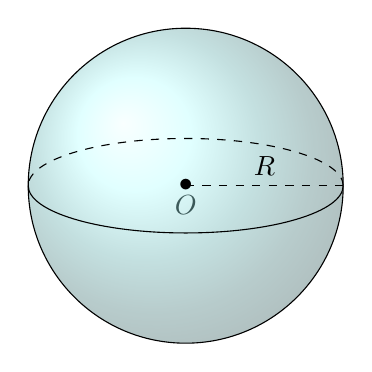
\begin{tikzpicture}
		\coordinate[label=below:$O$] (O) at (0,0);
		\shade[ball color = cyan!40, opacity = 0.4] (0,0) circle (2cm);
		\draw (0,0) circle (2cm);
		\draw (-2,0) arc (180:360:2 and 0.6);
		\draw[dashed] (2,0) arc (0:180:2 and 0.6);
		\fill[fill=cyan] (0,0) circle (1pt);
		\draw[dashed] (O) -- node[above]{$R$} (2,0);
		\node at (O) {$\bullet$};
		\end{tikzpicture}
		\caption{ស៊្វែ}
	\end{figure}
\end{multicols}
\subsection{សមភាពនៃមុំ}
\begin{enumerate}[m]
	\item \emph{\kml មុំទល់កំពូល} 
	\begin{multicols}{2}
		បើយើងរកឃើញ $\angle M_{1}$ និង $\angle M_{2}$ ជាមុំទល់កំពូល \\យើងបានៈ $\angle M_{1}=\angle M_{2}$
		\begin{figure}[H]
			\centering
			\begin{tikzpicture}
			\coordinate[label=above left:$A$] (A) at (0,1);
			\coordinate[label=below right:$B$] (B) at (4,0);
			\coordinate[label=below left:$C$] (C) at (0,0);
			\coordinate[label=above right:$D$] (D) at (4,1);
			\coordinate[label=above:$M$] (M) at (2,.5);
			\draw (A) -- (B);
			\draw (C) -- (D);
			\node at (M) {$$};
			\pic [draw, -, "$1$", angle eccentricity=1.8] {angle = A--M--C};
			\pic [draw, -, "$2$", angle eccentricity=1.8] {angle = B--M--D};
			\end{tikzpicture}
			\caption{មុំទល់កំពូល}
		\end{figure}
	\end{multicols}
	\item \emph{\kml មុំមានជ្រុងកែងរៀងគ្នា} 
	\begin{multicols}{2}
		កាលណាយើងមានមុំពីរ $\angle x'ox$ និង $\angle y'oy$ ហើយយើងមានជ្រុង $ox'\perp oy'$ និង $ox\perp oy$។\\ យើងបាន $\angle x'ox=\angle y'oy$
		\begin{figure}[H]
		\centering
		\begin{tikzpicture}[scale=.8]
		\coordinate[label=above left:$x$] (A) at (0,0);
		\coordinate[label=below:$O$] (B) at (4,0);
		\coordinate[label=above left:$x'$] (C) at (1,2);
		\coordinate[label=left:$y$] (D) at (2.5,-1);
		\coordinate[label=above:$O$] (M) at (2.5,3);
		\coordinate[label=below:$y'$] (N) at (.2,-.5);
		\draw (A) -- (B)--(C);
		\draw (D) -- (M)--(N);
		\node at (M) {$$};
		\pic [draw, -, "$\theta$", angle eccentricity=1.8] {angle = C--B--A};
		\pic [draw, -, "$\theta$", angle eccentricity=1.8] {angle = N--M--D};
		\end{tikzpicture}
		\caption{ មុំមានជ្រុងកែងរៀងគ្នា}
	\end{figure}
	\end{multicols}
	\item \emph{\kml មុំដែលមានជ្រុងស្របរៀងគ្នា} 
	\begin{multicols}{2}
		បើ $ox\parallel o'x'$ និង $oy\parallel o'y'$ នោះមុំ $\angle xoy$ និង $\angle x'o'y'$ ហៅថាមុំមានជ្រុងត្រូវគ្នា ស្របរៀងគ្នាដែលមានតម្លៃស្មើគ្នា។ យើងបាន $\alpha=\theta$
		\begin{figure}[H]
			\centering
			\begin{tikzpicture}
			\coordinate[label=left:$O$] (A) at (0,0);
			\coordinate[label=left:$O'$] (B) at (0,2.5);
			\coordinate[label=below:$y'$] (C) at (4,2.5);
			\coordinate[label=above:$x'$] (D) at (3,4.5);
			\coordinate[label=below:$y$] (M) at (4,0);
			\coordinate[label=below:$x$] (N) at (3,2);
			\draw (C) -- (B)--(D);
			\draw (M) -- (A)--(N);
			\pic [draw, -, "$\theta$", angle eccentricity=1.5, angle radius=1cm] {angle = M--A--N};
			\pic [draw, -, "$\alpha$", angle eccentricity=1.5, angle radius=1cm] {angle = C--B--D};
			\end{tikzpicture}
			\caption{ មុំដែលមានជ្រុងស្របរៀងគ្នា}
		\end{figure}
	\end{multicols}
	\item \emph{\kml កន្លះបន្ទាត់ពុះមុំ} 
	\begin{multicols}{2}
		បើយើងរកឃើញថា $OI$ ជាកន្លះបន្ទាត់ពុះមុំ $\angle xoy$ នោះយើងបាន $\angle O_{1}=\angle O_{2}$។
		\begin{figure}[H]
			\centering
			\begin{tikzpicture}
			\coordinate[label=left:$O$] (A) at (0,0);
			\coordinate[label=above:$x$] (B) at (3,2);
			\coordinate[label=below:$y$] (C) at (3,-2);
			\coordinate[label=below:$I$] (I) at (4,0);
			\draw (B) -- (A)--(C);
			\draw (A) -- (I);
			\pic [draw, -, "$1$", angle eccentricity=1.5, angle radius=.6cm] {angle = I--A--B};
			\pic [draw, -, "$2$", angle eccentricity=1.5, angle radius=1cm] {angle = C--A--I};
			\end{tikzpicture}
			\caption{ កន្លះបន្ទាត់ពុះមុំ}
		\end{figure}
	\end{multicols}
		\item \emph{\kml មុំផ្គុំដោយបន្ទាត់ពីរស្របគ្នានិងខ្នាត់មួយ} 
		បើ $\left(d\right)\parallel\left(d'\right)$ និង $\left(\Delta\right)$ ជាខ្នាត់យើងបានៈ
		\begin{align*}
			\angle A_{1}=\angle B_{7},\quad \angle A_{2}=\angle B_{8}\quad\left(\text{មុំឆ្លាស់ក្នុង}\right)\\
			\angle A_{3}=\angle B_{5},\quad \angle A_{4}=\angle B_{6}\quad\left(\text{មុំឆ្លាស់ក្រៅ}\right)\\
			\angle A_{1}=\angle B_{5},~\angle A_{2}=\angle B_{6},~\angle A_{3}=\angle B_{7},~\angle A_{4}=\angle B_{8}~\left(\text{មុំត្រូវគ្នា}\right)\\
			\angle A_{1}=\angle A_{3},~\angle A_{2}=\angle A_{4},~\angle B_{5}=\angle B_{7},~\angle B_{6}=\angle B_{8}~\left(\text{មុំទល់កំពូល}\right)
		\end{align*}
		\begin{figure}[H]
			\centering
			\begin{tikzpicture}
			\coordinate[label=left:$$] (A) at (0,2);
			\coordinate[label=above:$d$] (B) at (3,2);
			\coordinate[label=below:$$] (C) at (3,-2);
			\coordinate[label=below:$$] (D) at (0,0);
			\coordinate[label=below:$d'$] (E) at (3,0);
			\coordinate[label=below:$$] (F) at (1,-1);
			\coordinate[label=above:$\Delta$] (G) at (2,3);
			\coordinate[label=above:$1$] (A1) at (1,0);
			\coordinate[label=above:$2$] (A2) at (1.5,0);
			\coordinate[label=above:$3$] (A3) at (1.4,-.6);
			\coordinate[label=above:$4$] (A4) at (.9,-.6);
			\coordinate[label=above:$5$] (B5) at (1.5,2);
			\coordinate[label=above:$6$] (B6) at (2.1,2);
			\coordinate[label=above:$7$] (B7) at (2.1,1.5);
			\coordinate[label=above:$8$] (B8) at (1.5,1.5);
			\coordinate[label=above:$A$] (I1) at (1.7,.3);
			\coordinate[label=above:$B$] (I2) at (2.3,2.4);
			\draw (A) -- (B);
			\draw (D) -- (E);
			\draw (F)--(G);
			\end{tikzpicture}
			\caption{ មុំផ្គុំដោយបន្ទាត់ពីរស្របគ្នានិងខ្នាត់មួយ}
		\end{figure}
	\item \emph{\kml មុំឈមប្រលេឡូក្រាម} 
		\begin{multicols}{2}
		បើយើងមានប្រលេឡូក្រាម $ABCD$ ដូចរូប។ យើងបាន $\angle A=\angle C,~\angle B=\angle D$ (មុំឈមប្រលេឡូក្រាម)
		\begin{figure}[H]
			\centering
			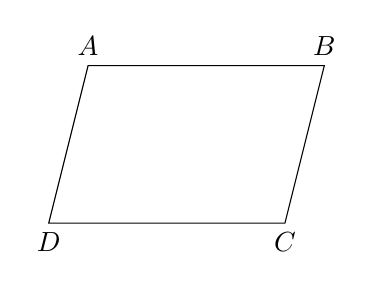
\begin{tikzpicture}
			\coordinate[label=below:$D$] (A) at (0,0);
			\coordinate[label=below:$C$] (B) at (3,0);
			\coordinate[label=above:$B$] (C) at (3.5,2);
			\coordinate[label=above:$A$] (D) at (.5,2);
			\draw (A)--(B)--(C)--(D)--cycle;
			\end{tikzpicture}
			\caption{ មុំឈមប្រលេឡូក្រាម}
		\end{figure}
\end{multicols}
\end{enumerate}
\subsection{តារាងមុំនៃអនុគមន៍ត្រីកោណមាត្រ}

\begin{center}
	\begin{tabular}{ | c | c | c | c | c | c | c | c | c | }
		\hline
		$\alpha\left(^\circ\right)$ & $0^\circ$ & $30^\circ$ & $45^\circ$ & $60^\circ$ & $90^\circ$ & $120^\circ$ & $135^\circ$ & $180^\circ$\\ \hline
		$\alpha\left(rad\right)$ & $0$ & $\frac{\pi}{6}$ & $\frac{\pi}{4}$ & $\frac{\pi}{3}$ & $\frac{\pi}{2}$ & $\frac{2\pi}{3}$ & $\frac{3\pi}{4}$ & $\pi$\\ \hline
		$\sin\alpha$ & $0$ & $\frac{1}{2}$ & $\frac{\sqrt{2}}{2}$ & $\frac{\sqrt{3}}{2}$ & $1$ & $\frac{\sqrt{3}}{2}$ & $\frac{\sqrt{2}}{2}$ & $0$\\ \hline
		$\cos\alpha$ & $1$ & $\frac{\sqrt{3}}{2}$ & $\frac{\sqrt{2}}{2}$ & $\frac{1}{2}$ & $0$ & $-\frac{1}{2}$ &$-\frac{\sqrt{2}}{2}$ & $-1$ \\
		\hline
	\end{tabular}
\end{center}
\begin{multicols}{2}
	ឧបមាថាយើងមានត្រីកោណកែង $ABC$ ដូចបង្ហាញក្នុងរូបខាងស្តាំ ។
	\begin{align*}
	\text{តាមពីតាគ័រ}\quad BC^{2}=BA^{2}+AC^{2}\\
	\sin\theta=\frac{\text{ជ្រុងឈម}}{\text{អុីប៉ូតេនុស}},\quad \cos\theta=\frac{\text{ជ្រុងជាប់}}{\text{អុីប៉ូតេនុស}},\quad \tan\theta=\frac{\text{ជ្រុងឈម}}{\text{ជ្រុងជាប់}}
	\end{align*}
	\begin{figure}[H]
		\centering
		\begin{tikzpicture}
		\centering 
		\begin{scope}
		\large
		\coordinate (C) at (0,0);
		\coordinate (A) at (3,0);
		\coordinate (B) at (3,2);
		\draw (C) -- (A) -- (B) -- cycle;
		\pic [draw, -, "$\theta$", angle eccentricity=1.5] {angle = A--C--B};
		\draw (A) -- ++ (0, .3cm) -- ++ (-.3cm, 0) -- ++ (0, -.3cm);
		\coordinate[label=below:$A$] (A) at (A);
		\coordinate[label=above:$B$] (B) at (B);
		\coordinate[label=below:$C$] (C) at (C);
		\coordinate[label=below:{\text{ជ្រុងជាប់}}] (1.5,0) at (1.5,0);
		\coordinate[label=right:{\text{ជ្រុងឈម}}] (3,1) at (3,1);
		\coordinate[label=right:{\text{អុីប៉ូតេនុស}}] (-1,1) at (-1,1);
		\end{scope}
		\end{tikzpicture}
		\caption{ទំនាក់ទំនងក្នុងត្រីកោណមាត្រ}
	\end{figure}
\end{multicols}
ទំនាក់ទំនង់រវាង $\sin\theta$ និង $\cos\theta$ គឺ
\begin{align*}
\tan\theta=\frac{\sin\theta}{\cos\theta} \quad \text{និង}\quad \sin^{2}\theta+\cos^{2}\theta=1
\end{align*}
\section{សមីការដឺក្រេទី២ មានមួយអញ្ញាត}
សមីការដឺក្រេទី២ មានរាងៈ $ax^{2}+bx+c=0$ ដែល $a$ ជាមេគុណទី១ $\left(a\ne0\right)$ $b$ ជាមេគុណទី២ និង $c$ ជាមេគុណទី៣ ហើយ $x$ ជាអញ្ញាត។\\
យើងអាចដោះស្រាយសមីការនេះបានដោយប្រើ ឌីសគ្រីមីណង់ $\Delta=b^{2}-4ab$។
\begin{center}
	\begin{tabular}{| c | c |}
		\hline
		 ឌីសគ្រីសមីណង់ & សមីការ​ $ax^{2}+bx+c=0~\left(a\ne 0\right)$ \\ \hline
		 បើ​ $\Delta = b^{2}-4ac>0$ & សមីការមានប្ញស $x_{1}, x_{2}=\frac{-b\pm\sqrt{\Delta}}{2a}$ (សមីការមានប្ញសពីរផ្សេងគ្នា) \\ \hline
		 បើ​ $\Delta = b^{2}-4ac=0$ & សមីការមានប្ញស $x_{1}= x_{2}=\frac{-b}{2a}$ (សមីការមានប្ញសឌុប) \\ \hline
		 បើ $\Delta = b^{2}-4ac<0$ & សមីការមានប្ញស $x_{1}, x_{2}=\frac{-b\pm i\sqrt{\Delta}}{2a}$ (សមីការមានប្ញសពីរជាចំនួនកុំផ្លិច) \\ 
		 \hline
	\end{tabular}
\end{center}
\begin{center}
	{\kml \Large \color{ magenta}ចប់ដោយសង្ខេប}
\end{center}